\subsection{Общая топология}

Раньше были телевизоры с \textit{бесконченым} количеством пикселей (это зависит от химических свойств вещества кинескоп).

\begin{center}
    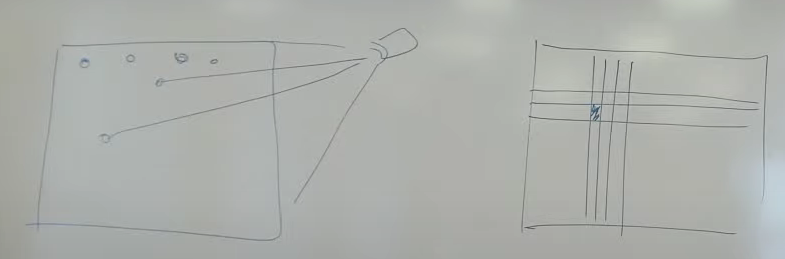
\includegraphics[scale=0.8]{img/topology_tv_example}
\end{center}

Возьмем множество $X$. Определим на нем топологию как подмножество множества всех подмножеств
$\Omega \subseteq \mathcal{P}(X)$. $\Omega$ --- топология, если это множество открытых множеств и выполнены следующие условия:
\begin{enumerate}
    \item $\varnothing, X \in \Omega$;
    \item $\bigcup\limits_i A_i \in \Omega$, если все $A_i \in \Omega$;
    \item $\bigcap\limits_{i = 1} ^ n A_i \in \Omega$, если $A_1, \dots, A_n \in \Omega$.
\end{enumerate}

То есть топологическое пространство~--- пара $\langle X, \Omega \rangle$ и про $\Omega$ верны приведенные выше три утверждения.

\begin{definition}
[Замкнутое мноежство] Множество $B$ такое, что $X \setminus B \in \Omega$ называется замкнутым.
\end{definition}

\begin{definition}
    [Связное топологическое пространство] $\langle X, \Omega \rangle$ связно, если нет $A, B \in \Omega ~:~ A \cup B = X$ и $A \cap B = \varnothing$
\end{definition}

\begin{definition}[Подпространство]
    $\langle X_1, \Omega_1 \rangle $ --- подпространство $\langle X, \Omega \rangle$, если
    $X_1 \subseteq X$ и $\Omega_1 = \{ a \cap X_1 ~|~ a \in \Omega$ \}
\end{definition}

\begin{definition}
    [Связное множество]

    Множество, являющееся связным подпространством.
\end{definition}

\begin{center}
    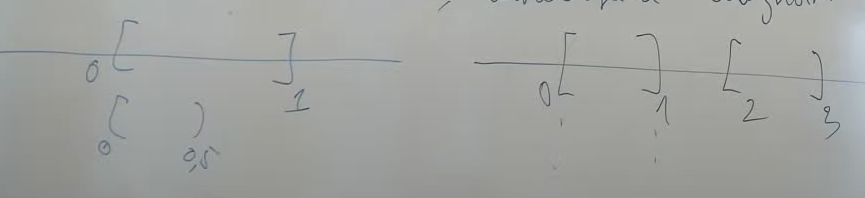
\includegraphics[scale=0.6]{img/topology_connectivy}
\end{center}

\subsection{Примеры топологических пространств}
Возьмем дерево (граф). Множество $X$~--- множество вержин. $\Omega$~--- множество всех вершин, что
$B \in \Omega$, \underline{если} $a \in B$, $x \leqslant a$ влечет $x \in B$.
То есть $\Omega$ --- семейство множеств вершин, которые входят вместе с поддеревом.

\begin{theorem}
    Граф без цикла свяен тогда и только тогда, когда оно своязно как топологическое пространство.
\end{theorem}
\begin{proof}[Доказательство будет в дз]
\end{proof}

\begin{definition}[Решетки]
    $X$~--- частично упорядоченное множество отношением $\leqslant$.\\
    Множество верхних граней $a, b$ $a \sqcap b$ --- множество $\{ x \in X ~|~ a \leqslant x, b \leqslant x\}$.\\
    Множество нижних граней $a, b$: $a \sqcup b$ --- множество $\{ x \in X ~|~ a \geqslant x, b \geqslant x\}$.\\
    $a$~--- наименьший элемент $A \iff$ $a \in A$ и любой $b \in A$, $b \geqslant a$.\\
    $a$~--- наибольший элемент $A \iff$ $a \in A$ и любой $b \in A$, $b \leqslant a$.\\
    $a+b$ = наименьший элемент множества верхних граний.\\
    $a \cdot b$ = наибольший элемент множества нижних граний.

    Решетка --- частично упорядоченное множество, где для каждых двух элементов существуют $a+b$ и $a \cdot b$.
\end{definition}

\begin{example}
    Дерево --- не решетка (в общем случае), так как $a + b$ есть, а $a*b$ может не быть.

    А вот такой граф является решеткой.

    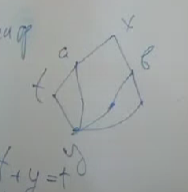
\includegraphics[scale=1]{img/grid_graph.png}
\end{example}

\begin{theorem}
    Пусть $\langle X, \Omega \rangle$ топологическое пространство, $A, B \in \Omega$. $A \leqslant B$, если $A \subseteq B$.

    Тогда $\langle \Omega, \leqslant\rangle$ --- решетка. $A \cdot B = A \cap B, ~ A + B = A \cup B$.
\end{theorem}

\begin{definition}
    Дистрибутивная решетка --- это такая решетка, что $a,b,c \in \Omega$, ~$a + (b \cdot c) = (a + b) \cdot (a + c)$.
\end{definition}

\begin{lemma}
    Для дистрибутивной решетки так же верно, что $a \cdot (b + c) = (a \cdot b) + (a \cdot c)$.
\end{lemma}

\begin{definition}
    Псевдодополнение $a \to b = \text{наибольшее} \{ c ~|~ a \cdot c \leqslant b\}$.
\end{definition}

\begin{definition}
    Диамант --- такая решетка, что там нет для кого-то псевдодополнения.

    \begin{center}
        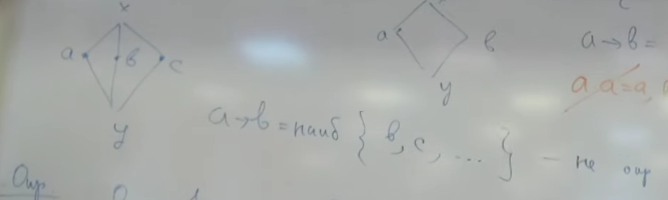
\includegraphics[scale=0.8]{img/topology_diomant}
    \end{center}
\end{definition}

\begin{definition}
    Решетка с псевдодополнением для всех элементов называется импликативной.
\end{definition}

\begin{definition} Определим 0 и 1 следующим образом:
    \begin{itemize}
        \item $0$ --- элемент, что $0 \leqslant x $ при всех $x$;
        \item $1$ --- элемент, что $x \leqslant 1 $ при всех $x$.
    \end{itemize}
\end{definition}

\begin{theorem}
    [В импликативной решетке 1 есть всегда] $\langle X, \leqslant \rangle$ --- импликативная решетка.
\end{theorem}
\begin{proof}
    Рассмотрим $a \to a= \text{наиб} \{ c ~|~ a \cdot c \leqslant a\} = \text{наиб} \{ X \} = 1$.
\end{proof}

\begin{theorem}
    Рассмотрим $\langle X, \Omega \rangle$ --- импликативная решетка с $0$. Рассмотрим И.И.В.


    Определим оценки $\mathbb{V}  = X$:
    \begin{itemize}
        \item     $\llbracket \alpha \& \beta \rrbracket = \llbracket\alpha \rrbracket \cdot \llbracket\beta \rrbracket$.
        \item     $\llbracket \alpha \vee \beta \rrbracket = \llbracket\alpha \rrbracket + \llbracket\beta \rrbracket$.
        \item     $\llbracket \alpha \to \beta \rrbracket = \llbracket\alpha \rrbracket \to \llbracket\beta \rrbracket$.
        \item     $\llbracket \neg \alpha \rrbracket = \llbracket\alpha \rrbracket \to 0$.
    \end{itemize}

    $\alpha$ истинно, если $\llbracket \alpha \rrbracket = 1$.

    $\llbracket\bot \rrbracket = 0$.
    $\neg \alpha \equiv \alpha \to \bot$.

    Полученная модель --- корректная модель И.И.В.
\end{theorem}

\begin{definition}
    Натуральный вывод~--- построение доказательства в виде дерева, где полученное утверждение в самом низу.
\end{definition}

$\overline{\Gamma, \varphi \vdash \varphi}$ (аксиома).

Вывод утверждения в доказательстве $\Gamma \vdash \varphi$.


Правила вывода (сверху~--- посылка, снизу~--- заключение):
\[
    \dfrac{\Gamma, \varphi \vdash \psi}{\Gamma \vdash \varphi \to \psi},~~~
    \dfrac{\Gamma, \varphi \vdash \psi~~~ \Gamma \vdash \varphi}{\Gamma \vdash \psi},~~~
    \dfrac{\Gamma, \varphi ~~~ \Gamma \vdash \psi}{\Gamma \vdash \varphi \& \psi},~~~
    \dfrac{\Gamma, \vdash \varphi \& \psi}{\Gamma \vdash \varphi},~~~
    \dfrac{\Gamma, \vdash \varphi \& \psi}{\Gamma \vdash \psi},
\]\[
    \dfrac{\Gamma \vdash \varphi}{\Gamma\vdash\varphi \vee \psi},~~~
    \dfrac{\Gamma \vdash \psi}{\Gamma\vdash\varphi \vee \psi},~~~
    \dfrac{\Gamma, \varphi \vdash \rho~~~ \Gamma, \psi \vdash \rho~~~ \Gamma \vdash \varphi \vee \psi}{\Gamma\vdash\rho},~~~
    \dfrac{\Gamma \vdash \bot }{\Gamma\vdash\varphi}.
\]

Вот они, слева направо: введение $\to$, исключение $\to$, введение $\&$, два исключения $\&$, введения $\lor$ в двух видах, исключение $\lor$ и специальное правило для лжи.

\begin{theorem}
    Если $\vdash_\text{И} \alpha \lor \beta$, то $\vdash_\text{И} \alpha$ или $\vdash_\text{И} \beta$.
\end{theorem}
\endinput
